%% COMPILE WITH XeLaTeX
\documentclass{beamer}

\usepackage{fontspec,calc}
\setmainfont[Mapping=tex-text]{Montserrat}
\let\sfdefault\rmdefault

\mode<presentation>
\title{Holo}
\subject{Minimalistic Configuration Management}
\author{Stefan Majewsky}
\date[32C3]{32nd Chaos Communication Congress, Hamburg, 2015}

\usetheme{default}
\beamertemplatenavigationsymbolsempty
\hypersetup{pdfpagemode=UseNone} % don't show bookmarks on initial view

\definecolor{holoonblack}{RGB}{0,199,255}

\setbeamercolor{titlelike}{fg=white,bg=black}
\setbeamercolor{normal text}{fg=white,bg=black}
\setbeamercolor{local structure}{fg=holoonblack}

\begin{document}

\begin{frame}[plain,c]
 \centering
 \LARGE Configuration management tools
\end{frame}

\begin{frame}[plain,t]{Optimized for huge systems}
 \centering
 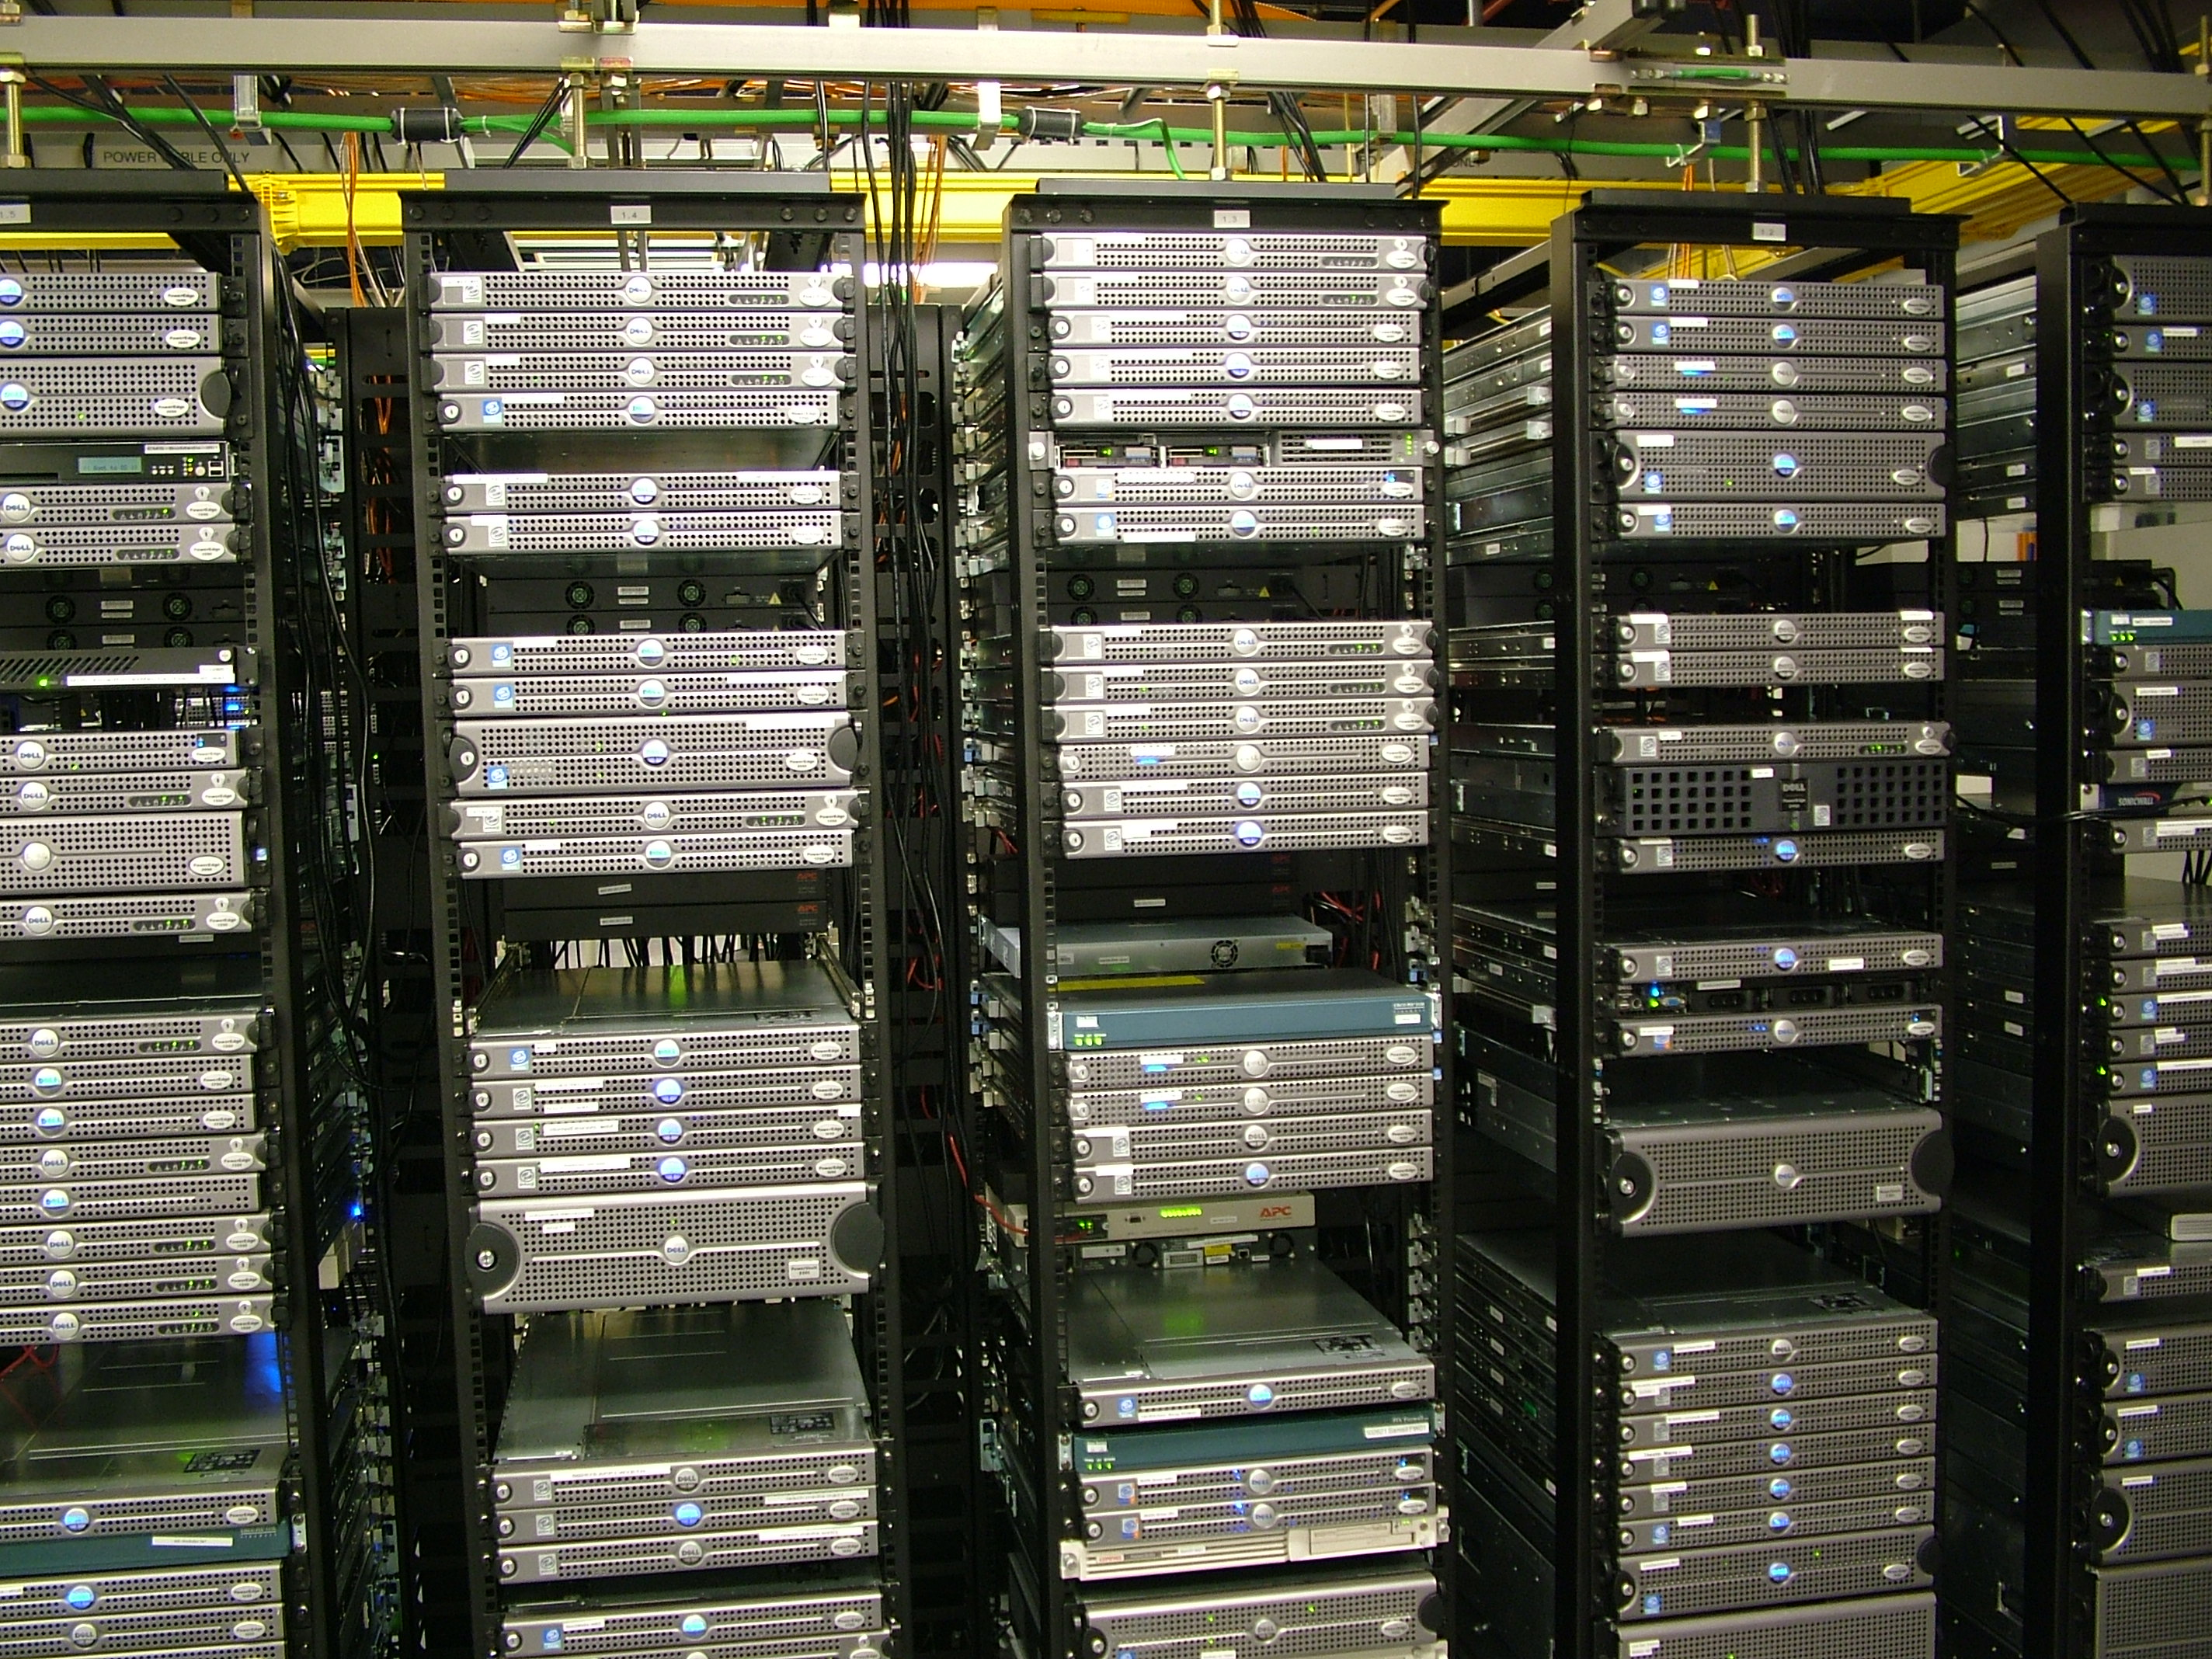
\includegraphics[height=0.8\textheight]{datacenter.jpg}
 \par\Tiny Image by NeoSpire, licensed under CC-BY 2.0, source: \url{https://www.flickr.com/photos/neospire/3595638270/}
\end{frame}

\begin{frame}[plain,t]{So they become huge systems themselves}
 \centering
 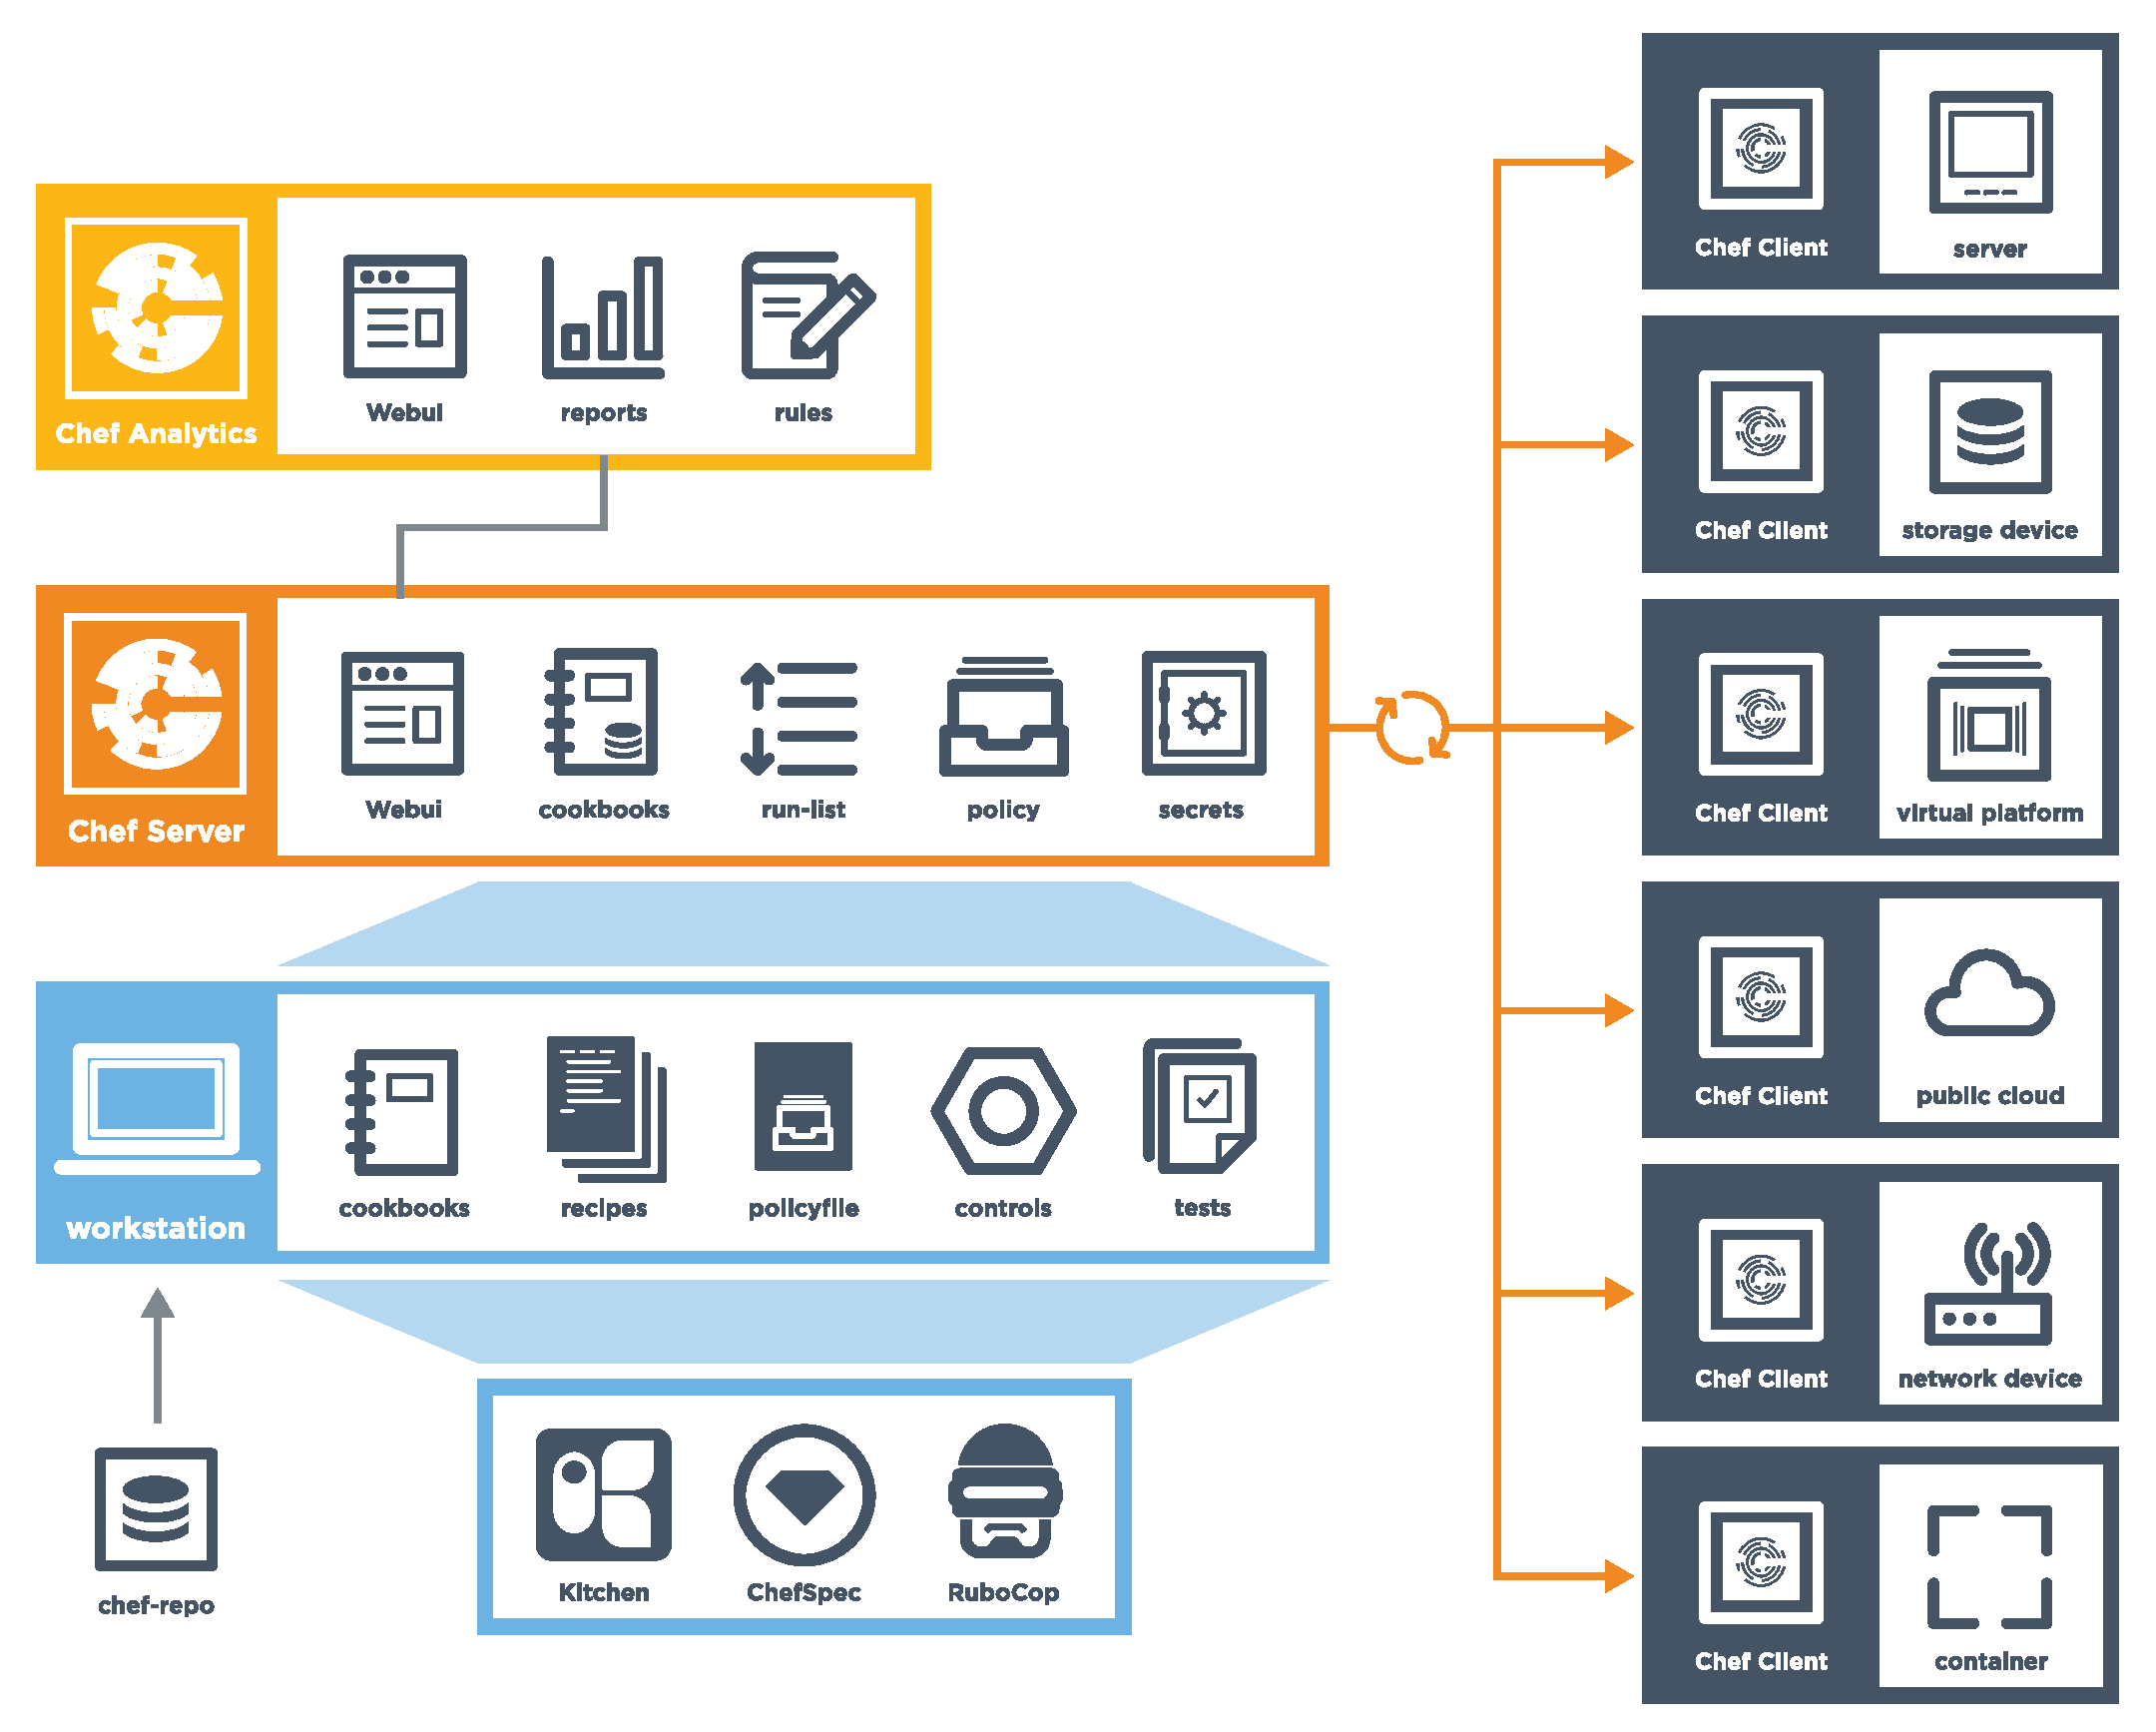
\includegraphics[height=0.8\textheight]{chef_overview.pdf}
 \par\Tiny Image from Chef documentation (authorship unknown), licensed under CC-BY 3.0 Unported, source: \url{https://docs.chef.io/chef_overview.html}
\end{frame}

\begin{frame}[plain,t]{My use-case is small}
 \centering
 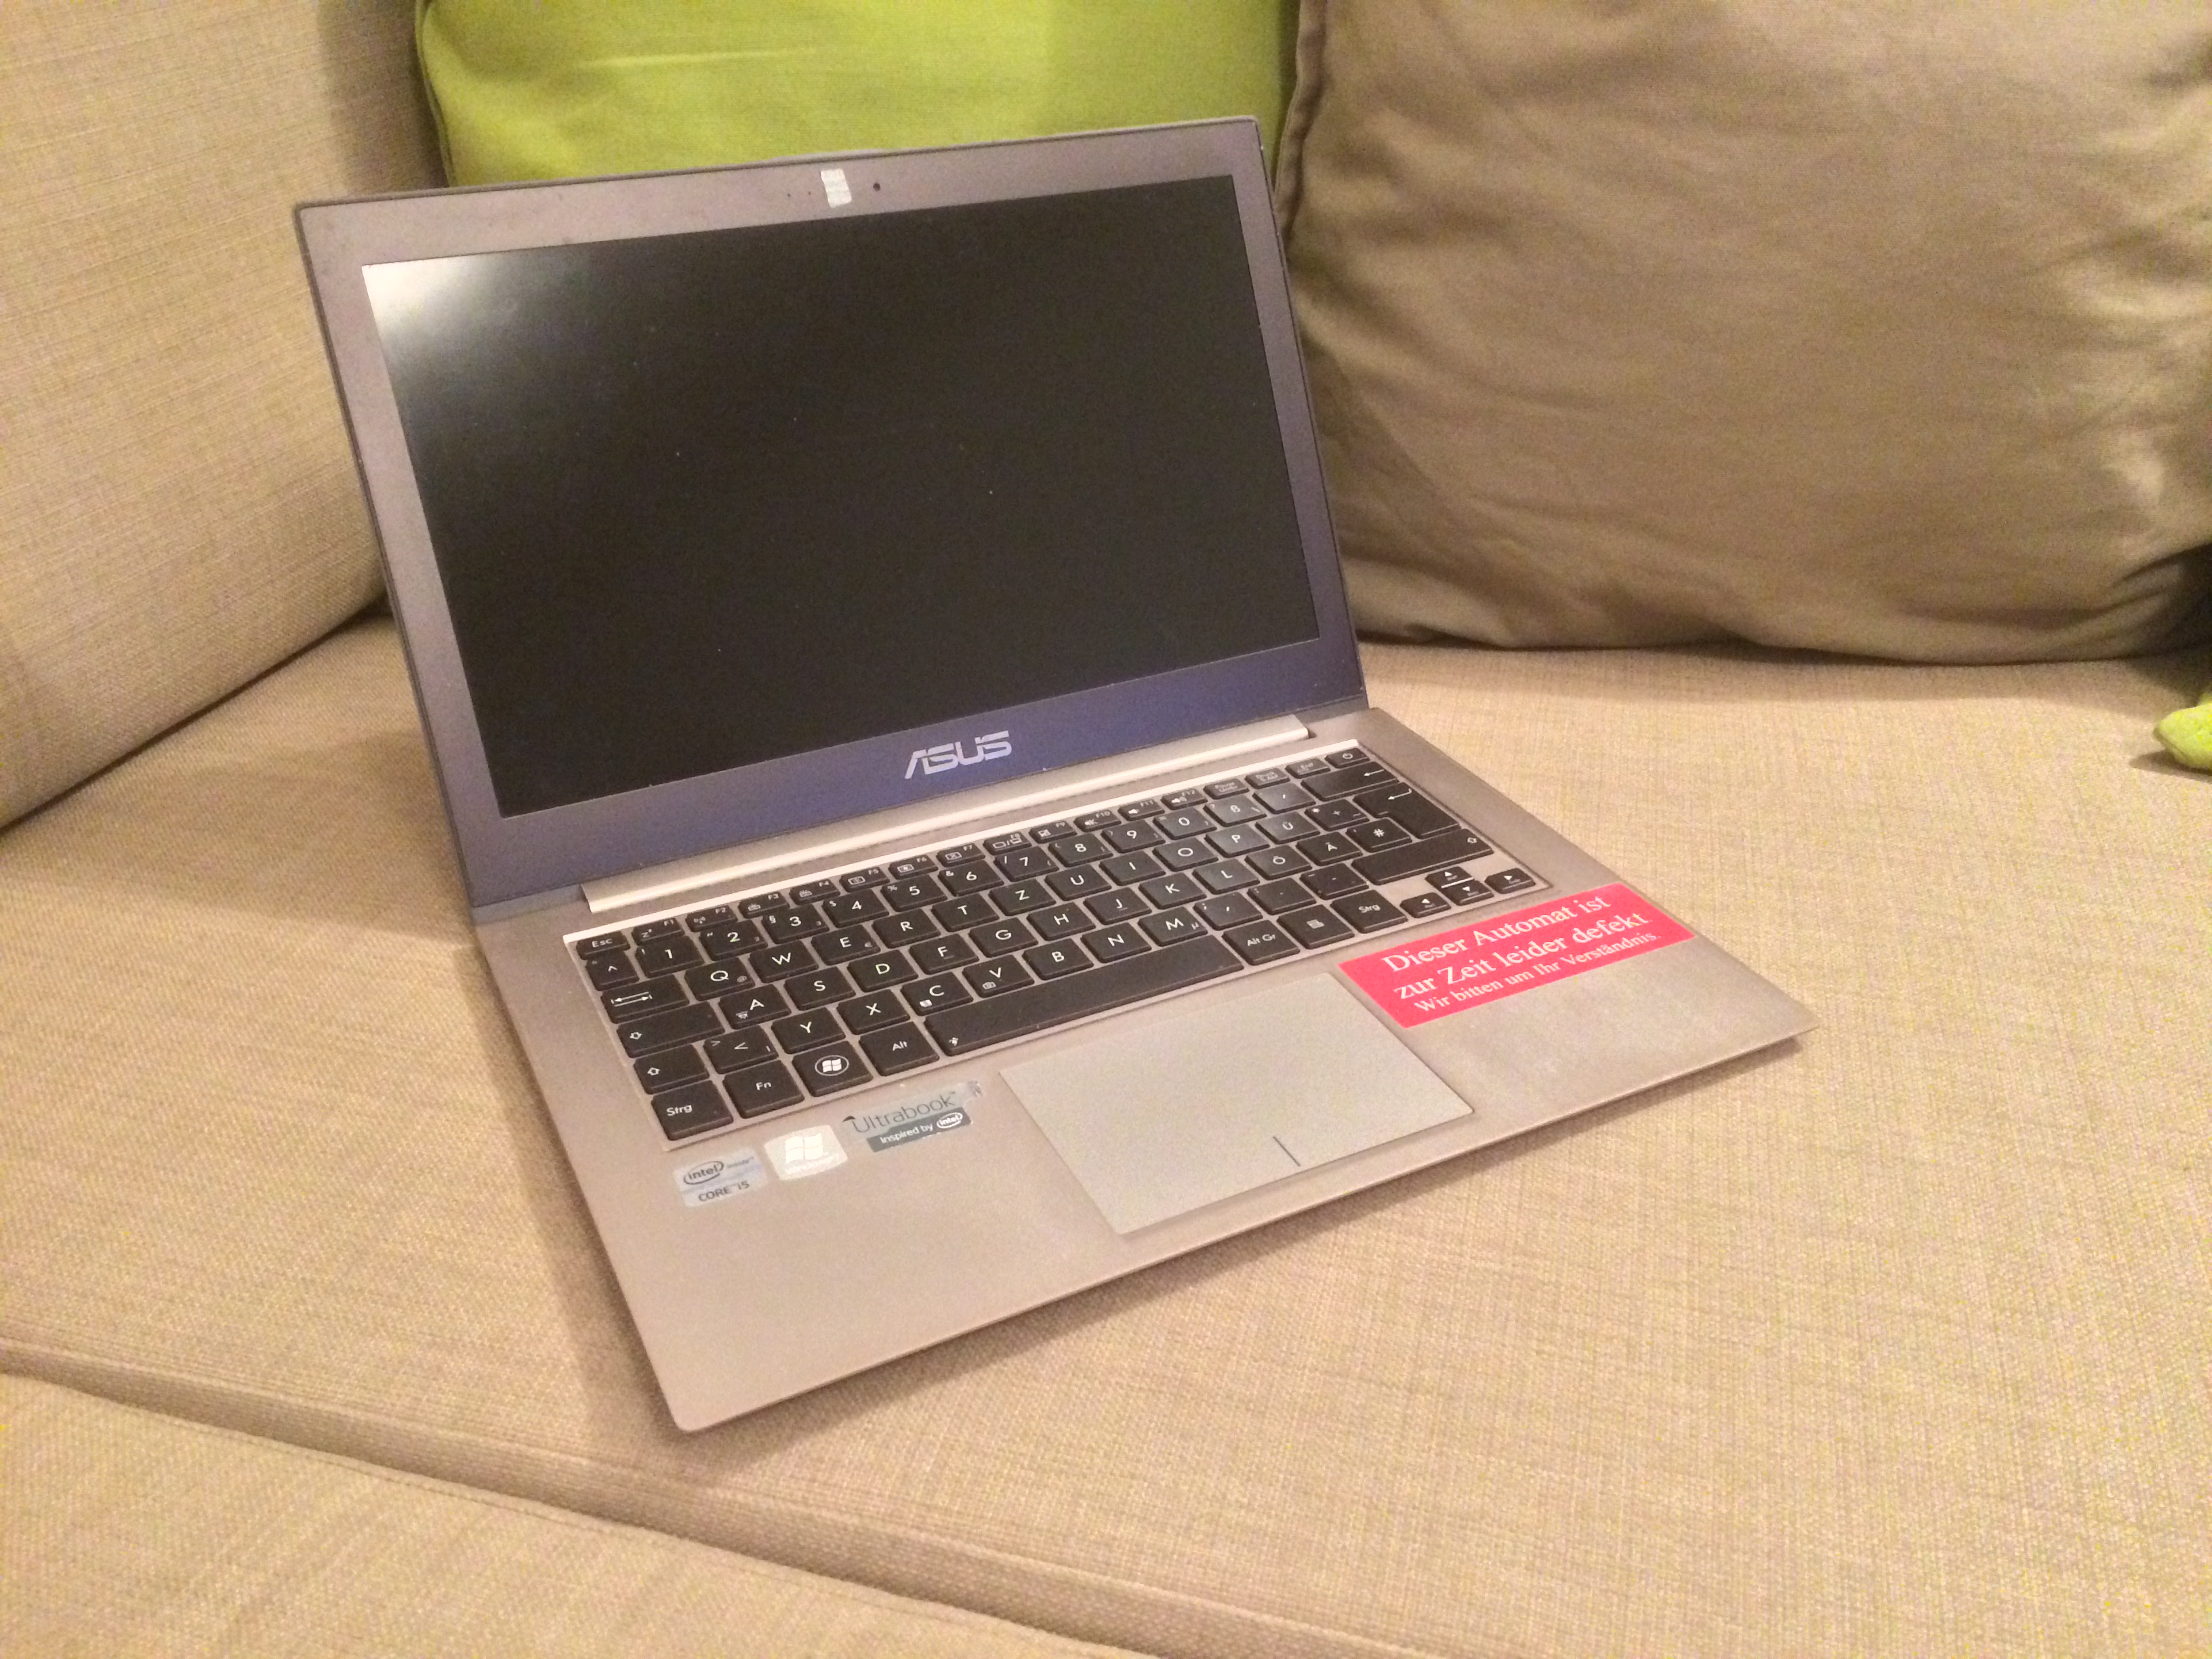
\includegraphics[height=0.8\textheight]{notebook.jpg}
\end{frame}

\begin{frame}[plain,c]
 \centering
 \LARGE Minimalistic configuration management
\end{frame}

\begin{frame}[plain,c]{Use the package manager!}
 \begin{itemize}
  \item list desired apps/daemons as dependencies
  \item put configuration files in the package
  \item setup users, groups, etc. in the post-install script
 \end{itemize}
\end{frame}

\begin{frame}[plain,t]{Limitations}
 \centering
 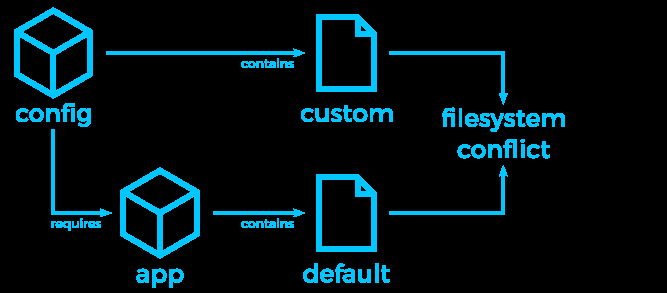
\includegraphics[width=\linewidth]{diagram-files2.pdf}
 \vspace{0em}
 \begin{itemize}
  \item File conflicts (as shown above)
  \item Detection of manual changes
 \end{itemize}
\end{frame}

\begin{frame}[plain,c]
 ~\vspace{3em}\par
 \centering
 
\includegraphics[width=0.7\textwidth]{holo-logo.pdf}
 \vspace{1em}\par\color{holoonblack}
 \small Holo builds on the package management of your Linux system and adds a minimal set of additional features to manage your system's configuration.
\end{frame}

\begin{frame}[plain,t]{Resolve file conflicts}
 \vspace{-1em}\begin{center}
  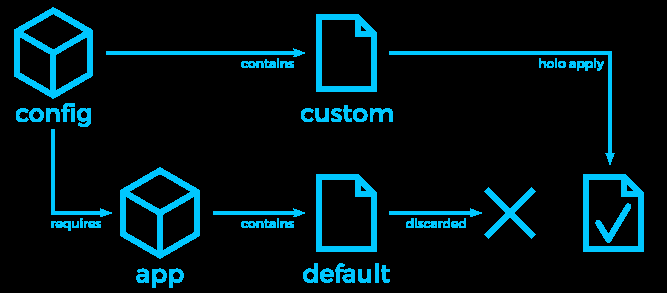
\includegraphics[width=\linewidth]{diagram-files3.pdf}
 \end{center}
 \begin{columns}\column{\dimexpr\paperwidth-15pt}
  \small\texttt{%
   {\color{holoonblack}\#} holo apply /etc/sudoers\\
   ~\\
   Working on \textbf{/etc/sudoers}\\
   ~~store at /var/lib/holo/files/base/etc/sudoers\\
   ~~~~~apply /usr/share/holo/files/50-config/etc/sudoers
  }
 \end{columns}
\end{frame}

\begin{frame}[plain,t]{Modify default configurations}
 \vspace{-1em}\begin{center}
  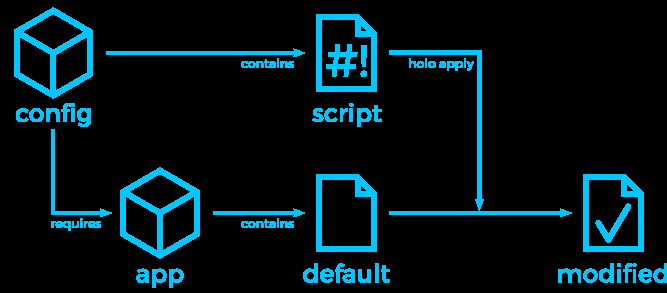
\includegraphics[width=\linewidth]{diagram-files4.pdf}
 \end{center}
 \begin{columns}\column{\dimexpr\paperwidth-15pt}
  \small\texttt{%
   {\color{holoonblack}\#} holo apply /etc/sudoers\\
   ~\\
   Working on \textbf{/etc/sudoers}\\
   ~~store at /var/lib/holo/files/base/etc/sudoers\\
   ~~passthru~/usr/share/holo/files/50-config/etc/sudoers.holoscript
  }
 \end{columns}
\end{frame}

\begin{frame}[plain,t]{Provision user accounts}
 \vspace{-1em}\begin{center}
  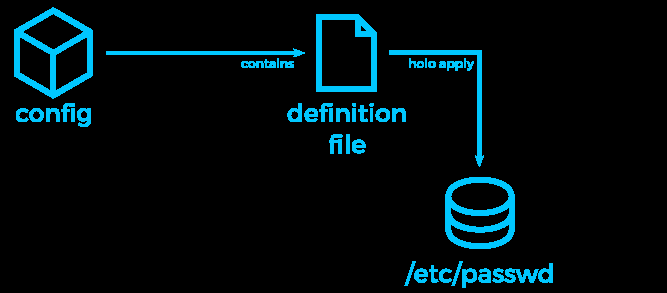
\includegraphics[width=\linewidth]{diagram-users.pdf}
 \end{center}
 \begin{columns}\column{\dimexpr\paperwidth-15pt}
  \small\texttt{%
   {\color{holoonblack}\#} holo apply user:stefan\phantom/\\
   ~\\
   Working on \textbf{user:stefan}\\
   ~~found in /usr/share/holo/users-groups/50-example.toml\\
   ~~~~~~with login group: users, login shell: /bin/zsh
  }
 \end{columns}
\end{frame}

\begin{frame}[plain,c]{Detect manual changes}
 \small\texttt{%
  {\color{holoonblack}\#} echo "PasswordAuthentication yes" >> /etc/ssh/sshd\_config\\[0.5em]
  {\color{holoonblack}\#} holo diff /etc/ssh/sshd\_config\\
  diff --git a/etc/ssh/sshd\_config b/etc/ssh/sshd\_config\\
  --- a/etc/ssh/sshd\_config\\
  +++ b/etc/ssh/sshd\_config\\
  @@ -146,3 +146,4 @@\\
  ~Ciphers~chacha20-poly1305@openssh.com,...\\
  ~\\
  ~MACs~hmac-sha2-512-etm@openssh.com,...\\
  +PasswordAuthentication yes\\[0.5em]
  {\color{holoonblack}\#} holo apply --force /etc/ssh/sshd\_config
 }
\end{frame}

\begin{frame}[plain,c]{Check it out!}
 \begin{center}
  
\includegraphics[width=0.5\textwidth]{holo-logo.pdf}
 \end{center}

 \texttt{%
  ~~~~~~~~~~~~https://github.com/{\color{holoonblack}holocm}/holo\\
  ~~~~~~~~~~~https://twitter.com/{\color{holoonblack}holocm}\\
  ~~~~~~~~~~~~~~~~~~~~~~~~http://{\color{holoonblack}holocm}.org
 }

 \vspace{3em}
 \small Contribution opportunities:\vspace{-0.3em}
 \begin{itemize}
  \item build a Holo package for your distribution\vspace{-0.3em}
  \item develop new plugins
 \end{itemize}
\end{frame}

\end{document}
